\documentclass[tikz,border=0pt]{standalone}
\usepackage[T1]{fontenc}
\usepackage{mathptmx,amsmath}
\usetikzlibrary{arrows.meta}
\begin{document}
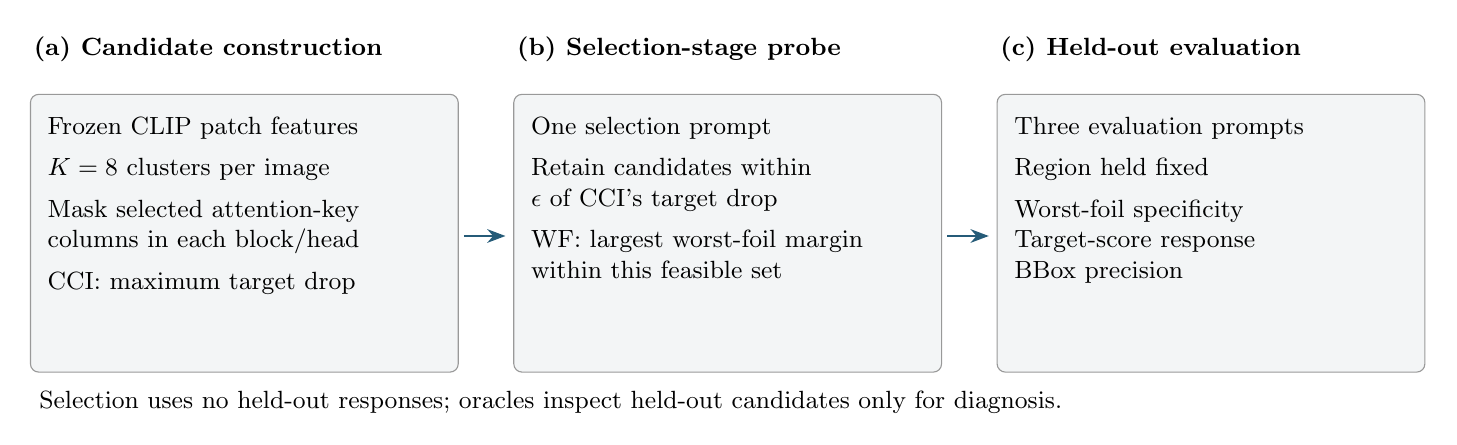
\begin{tikzpicture}[x=1bp,y=1bp,every node/.style={font=\fontsize{9.2}{11}\selectfont,align=left,inner sep=0},>=Stealth]
\path[use as bounding box] (0,0) rectangle (504.567,140);
\definecolor{ink}{HTML}{255B78}
\definecolor{pale}{HTML}{F3F5F6}
\foreach \x in {0,174,348}{\draw[draw=black!40,fill=pale,rounded corners=3] (\x+1,16) rectangle (\x+155,116);}
\node[anchor=north west,font=\fontsize{9.2}{11}\selectfont\bfseries] at (2,137) {(a) Candidate construction};
\node[anchor=north west,font=\fontsize{9.2}{11}\selectfont\bfseries] at (176,137) {(b) Selection-stage probe};
\node[anchor=north west,font=\fontsize{9.2}{11}\selectfont\bfseries] at (350,137) {(c) Held-out evaluation};
\node[anchor=north west,text width=142bp] at (7,108) {Frozen CLIP patch features\\[4pt]
$K=8$ clusters per image\\[4pt]
Mask selected attention-key\\columns in each block/head\\[4pt]
CCI: maximum target drop};
\node[anchor=north west,text width=142bp] at (181,108) {One selection prompt\\[4pt]
Retain candidates within\\$\epsilon$ of CCI's target drop\\[4pt]
WF: largest worst-foil margin\\within this feasible set};
\node[anchor=north west,text width=142bp] at (355,108) {Three evaluation prompts\\[4pt]
Region held fixed\\[4pt]
Worst-foil specificity\\Target-score response\\BBox precision};
\draw[->,thick,ink] (157,65)--(172,65);
\draw[->,thick,ink] (331,65)--(346,65);
\node[anchor=west] at (4,5) {Selection uses no held-out responses; oracles inspect held-out candidates only for diagnosis.};
\end{tikzpicture}
\end{document}
